\section{Anatomy}\label{sec:anatomy}

\begin{wrapfigure}{R}{0.3\textwidth}
    \centering
    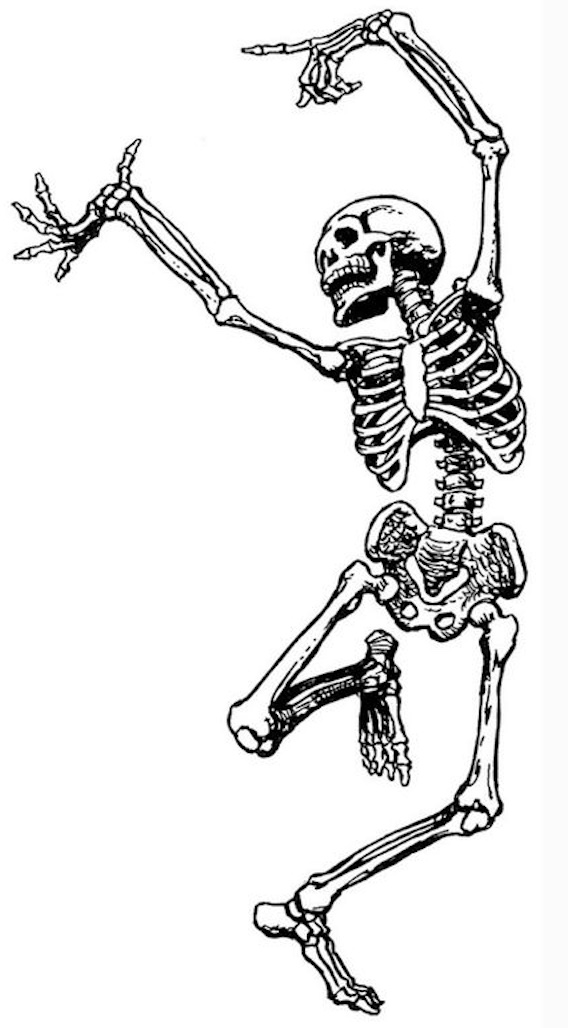
\includegraphics[width=0.25\textwidth]{images/anatomy}
\end{wrapfigure}

As with every system dealing with the human body, a basic understanding of the human anatomical body is unavoidable and adds a tremendous benefit for the practice but also when it comes to communicating certain aspects to others.
Because of that it is considered to be useful to also have a few, hand-picked, basic concepts also written here to familiarize yourself with them.

\subsection{Terminology}\label{subsec:terminology}

In order to understand the following, it is mandatory to be familiar with some basic terms used in medical anatomy.

\subsubsection{Orientation}

\begin{itemize}
    \setlength\itemsep{0em}
    \item anterior/posterior = front/back
    \item ventral/dorsal = front/back of the torso
    \item superior/inferior = above/below
    \item cranial/caudal = head-/tail-wards
    \item proximal/distal = towards to/away from center
    \item medial/lateral = towards/away the midline
    \item superficial/profund = more away/inside the body
\end{itemize}

\subsubsection{Movements}

\begin{itemize}
    \setlength\itemsep{0em}
    \item extension/flexion = making the angle of a joint (elbow, knee) bigger/smaller
    \item internal/external rotation = straight arm/leg rotating in the shoulder/hip join; alias medial/lateral rotation
    \item adduction/abduction = moving towards or away the body/midline
    \item elevation/depression = moving superior/inferior direction (e.g. shoulder shrug/lowering)
    \item pronation/supination = forearm rotating palm down/palm up (not same as rotation)
    \item dorsi-/plantarflexion = ankle only; moving towards the dorsum (superior surface) or plantar (sole) alias "point"
    \item in-/eversion = ankle only; sole towards/away the median plane, so they face medial/lateral direction
    \item opposition/reposition = thumb and little finger together/away from each other
    \item circumduction = conical (not really circular) movement of a limb extending from the joint its moved by
    \item pro-/retraction = anterolateral/posteromedial movement of scapula (move shoulder forward/backward)
\end{itemize}

\subsection{Structures}\label{subsec:structures}

\subsubsection{Bones}

\begin{itemize}
    \setlength\itemsep{0em}
    \item atlas and axis = two top most cervical vertebra
    \item clavicula = collar bone
    \item coccyx = tailbone (last part of the sacrum)
    \item cranium = skull (cervical = neck)
    \item spina = spine
    \item patella = kneecap
    \item processus = a bony thing bulging out, usually for tendons to attach to
    \item ribs = true (1-7, sternum connection), false (8-10/12, cartillage), floating (11-12, no connection)
    \item SIAS = Spina Illiaca Anterior Superior (front top pelvis bone)
    \item sternum = chest bone
\end{itemize}

\subsubsection{Muscles}

\begin{itemize}
    \setlength\itemsep{0em}
    \item gluteus = buttock (maximus, medius, minimus)
    \item diaphgragm = muscle for breathing bottom of ribs
    \item pectoralis = chest muscle
    \item pelvic floor = similar to diaphragm but at the bottom of the torso
    \item trapezius = top shoulder around the neck
\end{itemize}

\subsection{Planes}\label{subsec:planes}

\begin{wrapfigure}{R}{0.3\textwidth}
    \centering
    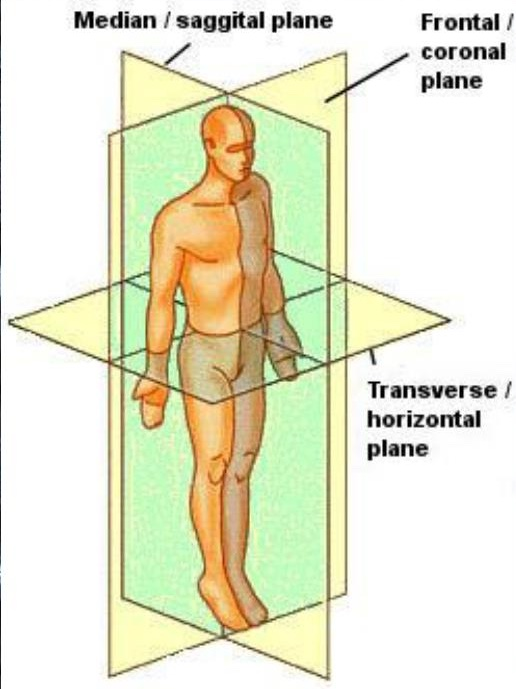
\includegraphics[width=0.25\textwidth]{images/anatomy_planes}
    \caption{The three anatomic planes for the human body: Frontal, Sagittal and Transversal.}
\end{wrapfigure}

We differentiate three different anatomical planes in which movement can happen:

\begin{enumerate}
    \setlength\itemsep{0em}
    \item \textbf{Frontal Plane}: Also called \textit{Coronal Plane} or \textit{Vertical Plane} and, not surprisingly, represents the plane when looking from the front of the body, dividing the body in an anterior/posterior part.
    The directions can be medial/lateral thus resulting in the movements of: ad-/abduction, elevation/depression and in-/eversion.
    \item \textbf{Sagittal Plane}: Also called \textit{Lateral Plane}, \textit{Longitudinal Plane} or \textit{Anteroposterior Plane}, which is going through the midline and shows the body when looking from the side, separating it into a left/right part.
    The directions are thus anterior/posterior and movements are flexion/extension and pro-/retraction.
    \item \textbf{Transverse Plane}: Also called \textit{Axial Plane}, \textit{Horizontal Plane} (the other two planes are vertical) or \textit{Cross-Sectional Plane}, and divides the body into a top/bottom part.
    Directions are thus superior/inferior and allowing movements like rotation, supination/pronation and circumduction.
\end{enumerate}


\subsection{Joints}\label{subsec:joints}

Bones are connected through joints where muscles (together with tendons) can evoke movement.
For different movements, different types of (synovial) joints are needed.

\begin{itemize}
    \setlength\itemsep{0em}
    \item Ball/Socket: hip, shoulder; free movement
    \item Pivot: head (atlantoaxial), elbow (radioulnar); rotation only
    \item Hinge: elbow (humeroulnar), knee, ankle; usually flexion/extension
    \item Saddle: fingers-hand (trapeziometacarpal)
    \item Condyloid: between fingers/wrist (metacarpophalangeal)
    \item Plane: hand (intercarpal) and feet (tarsal)
    \item Gliding: Foot mini bones
\end{itemize}
